\clearpage

\section{绪论}

\subsection{研究背景及意义}
在半导体材料制备领域，MBE作为原子级精度的薄膜制备技术，其核心优势在于能够通过反射式高能电子衍射RHEED技术，实现半导体材料制备过程中的衬底表面监测。RHEED通过高能电子束与晶体表面的相互作用产生动态衍射图谱，其图像特征能够精确反映原子层级的表面重构、生长模式转变及量子结构演化等关键信息\upcite{c1}。传统的RHEED图像分析方法高度依赖研究员的经验积累，通过肉眼识别衍射条纹或RHEED振荡曲线周期来推断衬底薄膜制备的生长参数，存在主观性强、响应滞后和无法处理高维度时序数据等缺陷，难以满足半导体器件制备对工艺可控性的严苛需求。近年来，随着MBE设备数字化升级和高速成像技术的突破，单次衬底薄膜MBE实验产生的RHEED图像和视频序列，为深度学习模型的应用提供了数据基础，同时也对传统计算机视觉方法提出了新挑战，如何从动态、多尺度、强噪声的RHEED图像序列中提取有效特征，并建立其与衬底薄膜生长参数的映射关系。

已有研究从不同角度验证了基于机器学习的RHEED图像智能分析具有可行性与潜在工程价值。Kwoen等针对MBE生长过程采集的RHEED图像构建数据集，利用CNN实现对典型表面重构模式的自动分类，在GaAs表面$(2×4)$与$c(4×4)$模式识别任务中取得很高的识别精度，验证了深度模型能够从衍射图像中学习到与表面结构相关的判别特征，从而降低人工经验依赖并具备实时反馈的应用前景\upcite{c1}，其后续工作进一步将二分类扩展到多类别RHEED模式，比如引入量子点生长相关的衍射特征等，仍保持高精度并具有较快推理速度，进一步验证了基于深度学习的RHEED模式识别可在更复杂的生长阶段中稳定工作，但跨设备、跨材料以及观测条件变化下的泛化能力仍是制约其工程部署的重要因素\upcite{c8}。与此同时，Yoshinari等提出skill-agnostic的分析思路，采用聚类与矩阵分解等无监督方法对Si(111)表面超结构的RHEED序列进行自动分段与相变检测，使其在较少人工干预下识别多种表面重构相，提示RHEED图像序列中蕴含的大量空间—时间信息仍有待系统挖掘\upcite{c9}。因此，面向RHEED图像强噪声、遮挡、动态演化、标注昂贵的数据特性，构建可复用的表征学习机制与更稳健的多任务协同分析框架，对于提升MBE设备自动化解析RHEED图像的能力、支撑MBE工艺实时反馈与智能调控具有重要意义。

图像分类作为计算机视觉的基础任务，其核心目标是输入图像，为其分配对应的语义标签。传统图像分类方法，多是基于卷积神经网络（Convolutional Neural Network , CNN）的架构优化，如视觉几何组网络（Visual Geometry Group Network, VGGNet）、残差网络（Residual Network, ResNet）等，传统分类方法受限于监督学习对标注数据的依赖。ConvNeXt V2通过结合全卷积掩码自编码器（Fully Convolutional Masked Autoencoder, FCMAE）与改进的全局响应归一化（Global Response Normalization, GRN）方法，提出了一种基于CNN架构的自监督学习框架\upcite{c2}。结合 RHEED 图像序列强噪声、部分图像存在遮挡等不利因素，本文在图像分类方法选择ConvNeXt V2，有效地克服了数据标注困难、成本高等问题。同样作为计算机视觉基础任务的目标检测，其核心任务是在一个图像中预测一组边界框和边界框对应的类别标签，传统的目标检测方法主要依赖于经验设计的候选框，通过回归和分类定位目标，但其固定候选机制导致训练与推理需严格匹配框数量，难以适应动态场景，如早期Regions with CNN features（R-CNN）的滑动窗口\upcite{c3,c4}、Faster Regions with CNN features（Faster R-CNN）\upcite{c5}的区域提议（region proposals）和You Only Look Once（YOLO）的锚框（anchor boxes）\upcite{c6}等。与传统目标检测方法不同的是，DiffusionDet将目标检测的视觉任务转换为图像去噪任务\upcite{c7}，从随机噪声框出发，通过多步迭代优化框的位置和尺寸，无需依赖手工设计的候选框或固定查询，在推理时可动态调整候选框的数量以捕捉密集目标，并利用迭代优化逐步修正噪声干扰下的检测偏差，适合RHEED图像中条纹和斑点数量复杂多变的目标检测场景。本文主要研究基于多任务深度学习框架，实现RHEED图像的分类、目标检测和RHEED震荡曲线时间序列预测，旨在建立图像分类、目标检测和时序预测联动的RHEED图像分析系统，为MBE工艺提供实时反馈，推动半导体材料生长从经验试错向智能调控范式的转变。

%自动编号公式示例，即公式后带（1-1）编号
% \begin{equation}
% \end{equation}


% %图片 pdf格式 测试
% 如图\ref{fig:w-xxx}所示

%  \begin{figure}[h]
%     \centering
%     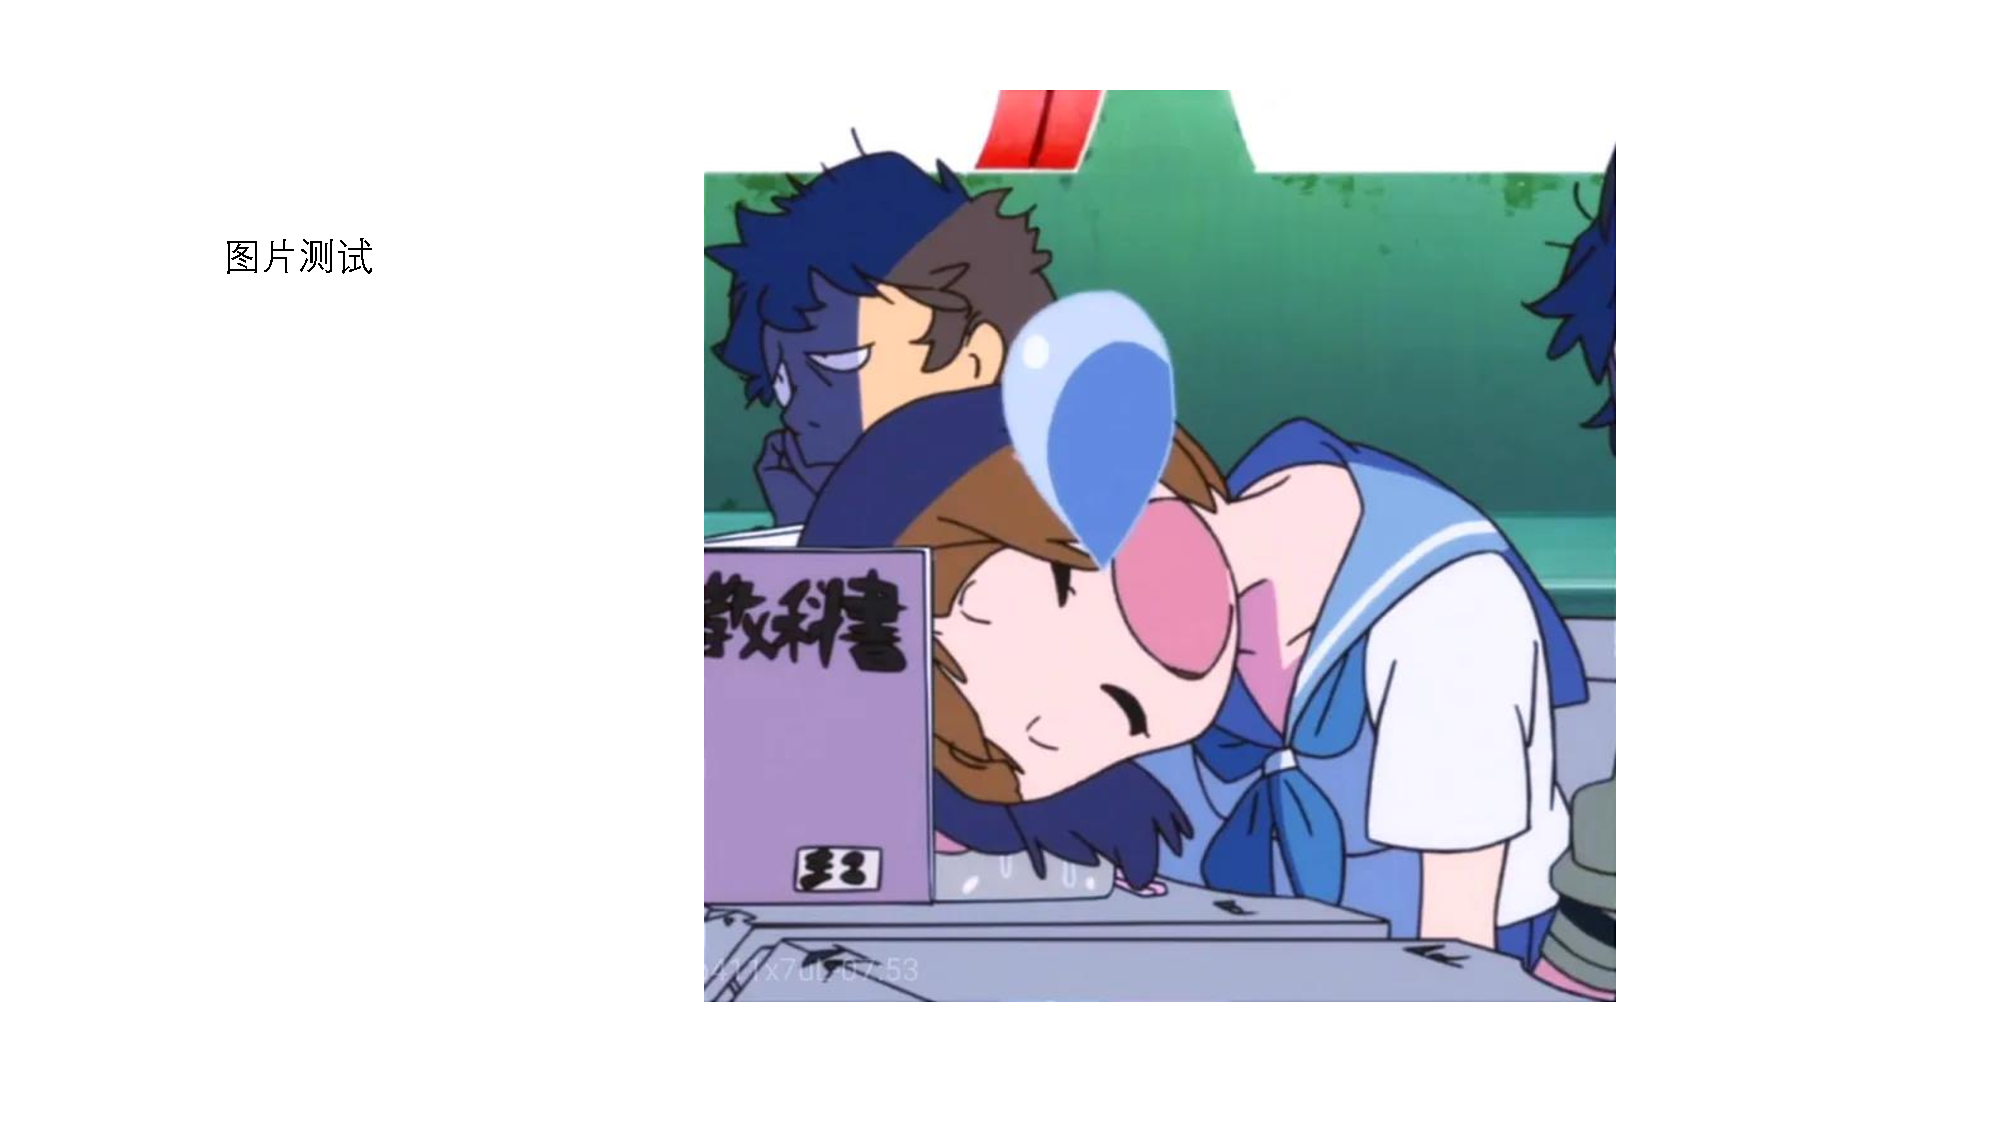
\includegraphics[width=0.8\textwidth]{figure/cp1/xxx.pdf}
%     \caption{11111}  
%     \label{fig:w-xxx}
%  \end{figure}


% 如表\ref{tab:xxx}所示

% % 表格测试 input插入
% \input{tables/EXP}

\subsection{国内外研究现状}
近年来，国内外学者围绕RHEED图像的特征提取、模式分类与动态监测等方向，开展了多层次的方法研究。现有研究主要基于无监督学习方法实现RHEED图像特征降维，并对其进行模式识别，例如，Gemperline等人\upcite{c10}通过主成分分析（Principal Component Analysis, PCA）和k-means聚类对薄膜生长中的RHEED图像序列进行定量分析，提出漂移校正和强度变换等图像预处理方法以增强RHEED图像菊池带（Kikuchi lines）等细微特征；Yoshinari团队\upcite{c9}则采用层次聚类和非负矩阵分解（Non-negative Matrix Factorization, NMF）方法分析硅衬底表面超结构的RHEED图像序列，对其进行自动相变检测，成功识别出5种表面重构相。上述方法虽能实现数据驱动的特征提取，但依赖人工设计图像的预处理流程。随着深度学习的发展，基于CNN的监督学习方法也成为新的研究方向，Kwoen等人\upcite{c10}采用CNN实现了砷化镓$2×4$与$center4×4$表面重构的二元分类，验证了CNN在静态模式识别中的有效性；Shen团队\upcite{c11}通过3DResNet模型处理RHEED图像序列，首次实现了量子点密度的实时反馈控制；Khaireh-Walieh团队\upcite{c12}利用自编码器（Auto-Encoder, AE）架构, 完成了RHEED图像的特征提取，并且结合有监督卷积分类器网络，在将RHEED图像压缩成潜在维度$N≥10$的向量和对应图像序列长度$L≥5$的先验条件下，对RHEED图像序列衬底是否脱氧的分类误差准确到了$1\%$以下。上述研究方法表明，基于CNN的监督学习方法在RHEED图像特征提取、时序演化建模等单任务场景中展现出强大潜力，但上述模型多针对特定的MBE设备或材料生长体系开发，且依赖大规模标注数据。
综上，目前RHEED图像分析方法的研究存在较多局限性：其一，针对无监督学习方法进行RHEED图像模式识别，需要复杂的预处理流程，如漂移校正、像素归一化、Region of Interest（ROI）裁剪，并且预处理的参数设置高度依赖MBE科研人员的经验，例如研究\upcite{c10}需要根据晶体表面的对称性人工确定RHEED图像对称轴位置，以此来对其进行漂移校正；研究\upcite{c9}要求手动划定RHEED荧光屏的有效区域等，这种人工干预不仅降低分析效率，还可能导致RHEED图像特征信息丢失，限制了算法在MBE动态环境中的鲁棒性。其二，针对有监督学习方法，存在数据标注依赖性强和模型泛化能力不足的挑战，例如研究\upcite{c8,c9,c13}普遍依赖人工标注的RHEED图像数据集，但如研究\upcite{c11}所述，RHEED图像动态变化复杂，人工标注成本高且易引入主观误差，研究\upcite{c11,c13}中还提到，基于特定MBE设备或材料训练的模型难以直接迁移到其他MBE设备或材料，需要重新标注训练数据集，缺乏普适性。

\subsection{本文的主要研究内容}
针对现有阶段已有的RHEED图像分析方法存在数据标注依赖性强、模型泛化能力不足和缺乏普适性等问题，本课题致力于研究一种多任务RHEED图像分析方法，解决上一小节所提出的关键挑战，其主要的研究内容及其创新总结如下：

（1）针对传统的基于监督学习的CNN，本课题提出ConvNeXt V2自监督学习框架实现RHEED图像分类，ConvNeXt V2提出基于FCMAE的自适应特征提取方法，通过FCMAE学习RHEED图像的全局语义特征，无需依赖人工进行复杂的图像预处理以增强RHEED图像菊池带（Kikuchi lines）等细微特征，其次，ConvNeXt V2引入了GRN方法，增强了RHEED图像弱特征的提取能力，有效地解决了传统CNN对噪声敏感的问题，此外，在少样本场景下（标注数据量少于$10\%$），ConvNeXt V2仍能保持高分类精度，可以显著降低本课题数据标注对MBE科研人员经验的依赖。

（2）针对传统的基于锚框的目标检测方法，本研究提出DiffusionDet实现RHEED条纹和斑点的目标检测。在进行MBE时，衬底表面的状态先从光滑演变到粗糙，继而从粗糙演变到光滑的过程复杂多变，呈现出来的RHEED条纹和斑点大小不一致，DiffusionDet通过扩散模型从随机噪声框中逐步优化检测的结果，有效地避免了人工设计锚框对RHEED条纹和斑点形态的假设偏差，其次，由于MBE设备存在机械臂的局限性，RHEED束打入衬底表面时存在被遮挡的情况，导致了RHEED图像序列中，存在遮挡、模糊的衍射斑点和条纹，DiffusionDet支持动态调整检测框数量，在MBE密集生长阶段或RHEED成像被遮挡情况，可自适应增加或减少目标检测的密度，提升了RHEED图像动态模式变化下，目标检测的鲁棒性。

（3）现有RHEED图像分析方法的研究中，单任务方法存在的特征割裂与泛化局限。本课题提出基于多任务协同的RHEED图像分析方法，该方法采用ConvNeXt V2骨干网络作为基础特征提取器，分类任务聚焦衬底表面全局重构状态的识别，进而分析MBE工艺下衬底薄膜生长阶段，目标检测任务引入DiffusionDet实现RHEED条纹和斑点密度的自适应定位。此外，在薄膜生长或表面重构过程中，包含的物理现象存在快速局部波动（原子级吸附或脱附的瞬态变化）和缓慢全局演变（晶格重构的周期性调整），快速局部波动需要高时间分辨率分析，而缓慢全局演变则需要低时间分辨率分析。本课题引入Pyraformer模型，通过时间多尺度建模实现 RHEED强度震荡曲线的时序预测任务。三个任务通过协同优化机制形成深度交互，分类任务输出的全局语义特征引导目标检测任务动态聚焦关键区域，而DiffusionDet生成的条纹和斑点空间分布特征可作为强度震荡曲线时序预测的先验约束，同时强度震荡曲线时序预测的动态信息可反向优化分类任务与目标检测任务的鲁棒性，对比单任务的RHEED图像分析方法，多任务可以有效提升其分析方法对跨设备和不同材料生长场景的适应性。

\subsection{本文的组织结构}
本文的结构共包含五个部分，具体安排如下：

第一章主要对本文研究的主要内容进行概述，梳理了现有RHEED图像分析方法的研究背景，总结基于深度学习方法分析RHEED图像的国内外研究现状。对现有方法中存在的问题进行分析，展示本文核心研究与创新内容。

第二章基于ConvNeXt V2方法对RHEED图像的分类任务展开讨论，对所提出方法的核心思想与创新点进行阐述，且详细描述方法中各个模块的运行原理。为了验证所提方法在RHEED图像分类中的有效性，设计了相关实验。

第三章基于DiffusionDet方法对RHEED图像条纹与斑点的检测任务展开讨论，结构设计与第二章类似。

第四章基于Pyraformer方法对RHEED强度震荡曲线时序预测任务展开讨论，结构设计与第二、三章类似。

第五章针对本研究的主要成果进行总结,和探讨后续可深入研究的方向，且提出值得进一步探索的若干研究问题。

